%%% The main file. It contains definitions of basic parameters and includes all other parts.


%% Settings for two-sided (duplex) printing
\documentclass[10pt,a4paper]{article}
\let\openright=\cleardoublepage

%% Character encoding: usually latin2, cp1250 or utf8:
\usepackage[utf8]{inputenc}

%% It's 2019
\usepackage[default]{droidserif}
\usepackage[T1]{fontenc}

%% Further useful packages (included in most LaTeX distributions)
\usepackage{amsmath}        % extensions for typesetting of math
\usepackage{amsfonts}       % math fonts
\usepackage{graphicx}       % embedding of pictures
\usepackage{tikz}
%\usetikzlibrary{shapes,fit,positioning,snakes,mindmap,trees,decorations.text,arrows.meta}
%\makenomenclature
\usepackage{algorithm,algpseudocode}
\usepackage{booktabs}
\usepackage{mwe}
\usepackage{afterpage}
\usepackage{pgfgantt}
\usepackage{pdflscape}
\usepackage{geometry}
\usepackage{enumitem}
\usepackage{float}
\usepackage{framed}
\usepackage{titlesec}
\usepackage{listings}
\usepackage{xcolor}
\usepackage{longtable}
\usepackage{makecell}
\usepackage[toc,page]{appendix}
\usepackage{multirow}
\usepackage{tocbibind}
\usepackage{etoolbox}
\usepackage{fancyvrb}
\usepackage{animate}

\lstset{basicstyle=\ttfamily,
	showstringspaces=false,
	commentstyle=\color{red},
	keywordstyle=\color{blue}
}

\usepackage{pdfpages}

\usepackage[textsize=tiny,backgroundcolor=yellow!50, linecolor=black!25]{todonotes}

% links shall be clickable
\usepackage[unicode]{hyperref}   % Must follow all other packages
\usepackage{cleveref} % Must follow all other packages including hyperref
\AtBeginEnvironment{appendices}{\crefalias{chapter}{appendix}}

% indexing
\usepackage{makeidx}
\makeindex
\usepackage[totoc, columns=1]{idxlayout}


\newcommand{\cool}{\color{green!50!white!80!black}}
\newcommand{\textcool}[1]{{\cool #1}}

\newcommand{\XX}[1]{\textcolor{red}{#1}}
\newcommand{\TT}[1]{\texttt{#1}}
\newcommand{\SC}[1]{{\fontfamily{phv}\selectfont\textsc{#1}}}

% Draw black "slugs" whenever a line overflows, so that we can spot it easily.


% avoid some slugs naturally
\clubpenalty=1000
\widowpenalty=1000
%\hyphenpenalty=100  % turn this on to prevent hyphenation
\emergencystretch=2cm


%%% The field of all real and natural numbers
\newcommand{\R}{\mathbb{R}}
\newcommand{\N}{\mathbb{N}}
\newcommand{\F}{\mathbb{F}}
\newcommand{\Z}{\mathbb{Z}}

\newcommand{\bms}{\begin{enumerate}[label=\bf (M\arabic*)]}
\newcommand{\bwp}{\begin{enumerate}[label=\bf \normalsize  (WP\arabic*), resume=del]}
\newcommand{\eenum}{\end{enumerate}}
\newcommand{\itemm}{\large \item }
\newcommand{\itemwp}{ \normalsize \item }
\newcommand{\deadline}[2]{\small (deadline: \textit{month #1}, duration: \textit{#2 moths})}
\newcommand{\people}[1]{\textit{\small (#1)}}


% move the headings out of gutenberg era
\setcounter{secnumdepth}{4}
\titleformat{\chapter}{\cool\fontsize{24pt}{24pt}\bfseries}{\color{black!25}\thechapter.}{1em}{}
\titleformat{\section}{\cool\fontsize{16pt}{18pt}\bfseries}{\scriptsize\color{black!25}\thesection}{1em}{}
\titleformat{\subsection}{\cool\fontsize{14pt}{16pt}\bfseries}{\scriptsize\color{black!25}\thesubsection}{1em}{}
\titleformat{\subsubsection}{\cool\fontsize{12pt}{14pt}\bfseries}{\scriptsize\color{black!25}\thesubsubsection}{1em}{}

% code floats
\colorlet{shadecolor}{cyan!10}
\makeatletter
\newcommand\floatc@code[2]{{\@fs@cfont #1} #2\par}
\newcommand\fs@code{\def\@fs@cfont{\bfseries}\let\@fs@capt\floatc@code
\def\@fs@pre{}%
\def\@fs@mid{\vspace{-.5ex}\begin{shaded}}%
\def\@fs@post{\vspace{-1em}\end{shaded}}%
\let\@fs@iftopcapt\iftrue}
\makeatother

\floatstyle{code}
\newfloat{listing}{tbp}{lst}
\floatname{listing}{Listing}

\title{\textcool{\bf High Level Assembler Plugin} \\ User documentation}
\author{Michal Bali, Marcel Hruška, Peter Polák,\\ Adam Šmelko, Lucia Tódová}
\date{Supervisor: Miroslav Kratochvíl \\ \vspace{5mm} Consultant: Slavomír Kučera (Broadcom)}

% Title page and various mandatory informational pages
\begin{document}
\maketitle
\pagebreak
%%% A page with automatically generated table of contents of the bachelor thesis
\tableofcontents

%%% Each chapter is kept in a separate file

\chapter{Introduction}

The IBM High Level Assembler Language (HLASM) is still actively used commercially, even though it is a relatively old language. Its roots go back to the 1970s, when IBM made their first mainframes. Since then, the IBM assembler has been revised several times --- the last version (which is the concern of this project) was released in 1992. Although it is hard to believe, a lot of the software that has been written in the language over the years is still actively used and maintained, mainly because of the conservative mainframe users and IBM's vendor lock-in.

Today, HLASM developers are forced to code in archaic terminals directly on the mainframe. Therefore, they spend a lot of time navigating around the code and the environment. For example, solely due to the fact that the user needs to navigate through plenty of terminal screens it takes around a minute just to get to a screen where it is possible to make a change in a file and recompile. For developers, it would be extremely useful to have an IDE plugin that would minimize contact with the mainframe terminal, could analyze the HLASM program, check its validity and make the code clearer by syntax highlighting. 

We introduce such plugin for Visual Studio Code, which is nowadays one of the most popular code editors. It improves HLASM programming experience, so that it can be compared to coding in modern programming languages, by providing instant code validity checks, advanced highlighting, code analysis, and all the functionality that a programmer currently takes for granted when writing code.

Some of the most noteworthy properties and features of the plugin are:
\begin{itemize}
	\item It is capable of interpreting and tracing a large subset of HLASM code-generating instructions
	\item It contains a list of all built-in instructions that is used to validate the generated code
	\item So called \emph{macro tracer} gives a possibility to trace the compilation of HLASM source code step-by-step in a way similar to common debugging.
	\item It implements DAP and LSP protocols, providing interface to be easily integrated into numerous modern code editors
	\item It has been run and tested on over 15 millions lines of real production HLASM code
\end{itemize}
The plugin is available on the Visual Studio Code Marketplace\footnote{\url{https://marketplace.visualstudio.com/items?itemName=broadcomMFD.hlasm-language-support}}

This document serves as an in-depth documentation for anyone who would like to understand the implementation of the project and the reasons behind it. It is advised that the potential contributors to the project read this documentation first.

User documentation is available on the Visual Studio Code marketplace \footnote{\url{https://marketplace.visualstudio.com/items?itemName=broadcomMFD.hlasm-language-support}} or in a markdown file \TT{clients/vscode-hlasmplugin/README.md}. The HLASM plugin project also contains an example workspace that can be used to test out the plugin.


\section{Organisation of this document}
First of all, in~\cref{hlasm}, we briefly explain the basics of HLASM needed to comprehend the workflow of this language. In~\cref{arch}, we provide an overview of the project's architecture, naming the most important components and indicating their relations. Then, we describe these components in separate chapters in further detail. In~\cref{chap:lang_server}, we state the responsibilities of the language server as the communication provider between the extension client and the parsing library. The workspace manager is the entry point to the parsing library used by the language server and it is fully described in~\cref{ws_manager}. The purpose of its sub-components is to handle file management, dependency resolution and parsing. The core of the processing of a HLASM file is implemented inside the analyzer, whose mechanics and implementation details are discussed in~\cref{chap:analyzer}. The project also provides macro tracing through the standard debugging procedure and it is fully explained in~\cref{macro_tracer}.The last mentioned component, detailed in~\cref{extension} is the VSCode extension, which communicates with the language server and provides IDE features to the user. At the end of this document, in~\cref{build}, we provide the instructions on how to build the project.

\chapter{Getting Started}

To start using the HLASM Language Support extension, follow these steps:

\begin{enumerate}
	\item Install the extension either from Visual Studio Marketplace\footnote{\url{https://marketplace.visualstudio.com/items?itemName=broadcomMFD.hlasm-language-support}} or from source as described in chapter 10 of the project documentation.
	\item In \textbf{File} - \textbf{Open Folder...}, select the folder where your HLASM project is located.
	\item Open your HLASM source code (no file extension is needed) or create a new file.
	\item If the extension fails to auto-detect HLASM language, set it manually in the bottom-right corner of the VS Code window.  
	\item The extension is now enabled on the opened file. If you have macro definitions in separate files or use the COPY instruction, proceed with the steps below to configure the extension to search for external files in the correct directories:
	\item After opening the HLASM file, two popups display. Select \TT{Create pgm\_conf.json with current program} and \TT{Create empty proc\_grps.json}. The two configuration files are created in the \emph{.hlasmplugin} subfolder.
	\item In the \emph{proc\_grps.json} file, fill the \emph{libs} array with paths to folders with macro definitions and COPY files. For example, if you have your macro files in the \emph{ASMMAC/} folder, type the string \emph{"ASMMAC"} into the libs array.
\end{enumerate}

There is an example workspace in the folder \TT{example\_workspace} that can be used to test out the extension.

For a full explanation of the configuration, see the~\cref{chap:configuration}.

\section{Functionality of extension}
\label{sec:features}
The HLASM Language Support extension parses and analyzes all parts of a HLASM program. It resolves all ordinary symbols, variable symbols and checks the validity of most instructions. The extension supports conditional and unconditional branching and can define global and local variable symbols. It can also expand macros and COPY instructions.

\subsection{Highlighting}
The HLASM Language Support extension highlights statements with different colors for labels, instructions, operands, remarks and variables. Statements containing instructions that can have operands are highlighted differently to statements that do not expect operands. Code that is skipped by branching AIF, AGO or conditional assembly is not colored.

\begin{figure}[h]
	\centering
	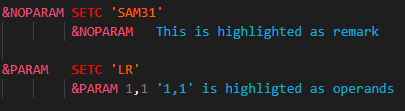
\includegraphics[width=10cm]{img/highligting}
	\caption{An example of highlighting.}
\end{figure}

\subsection{Autocomplete}
Autocomplete is enabled for the instruction field. While typing, a list of instructions starting with the typed characters displays. Selecting an instruction from the list completes it and inserts the default operands. Variables and sequence symbols are also filled with a value from their scope.

\begin{figure}[H]
	\centering
	\animategraphics[autoplay,loop,width=\linewidth]{12}{img/autocomplete/autocomplete-}{0}{126}
	\caption{\href{https://github.com/eclipse/che-che4z-lsp-for-hlasm/blob/master/readme\_res/autocomplete.gif}{Autocomplete usage example.}}
\end{figure}

\subsection{Go To Definition and Find All References}
The extension adds the functionality of \TT{go to definition} and \TT{find all references}. Use the \TT{go to definition} functionality to show definitions of variable symbols, ordinary symbols and macros, or open COPY files directly. Use the \TT{find all references} functionality to show all places where a symbol is used.

\begin{figure}[H]
	\centering
	\animategraphics[autoplay,loop,width=\linewidth]{12}{img/go_to_def/go_to_def-}{0}{90}
	\caption{\href{https://github.com/eclipse/che-che4z-lsp-for-hlasm/blob/master/readme\_res/go\_to\_def.gif}{Go To Definition usage example.}}
\end{figure}

\subsection{Macro Tracer}
The macro tracer functionality allows you to track the process of assembling HLASM code. It lets you see step-by-step how macros are expanded and displays values of variable symbols at different points during the assembly process. You can also set breakpoints in problematic sections of your conditional assembly code. 

The macro tracer is not a debugger. It cannot debug running executables, only track the compilation process.

\subsubsection{Configuring the Macro Tracer}

\begin{enumerate}
	\item Open your workspace.
	\item In the left sidebar, click the bug icon to open the debugging panel (Ctrl + Shift + D).
	\item Click create a launch.json file. A \TT{select environment} prompt displays.
	\item Enter \textbf{HLASM Macro tracer}. Your workspace is now configured for macro tracing.
\end{enumerate}

\subsubsection{Using the Macro Tracer}

To run the macro tracer, open the file that you want to trace. Then press \textbf{F5} to open the debugging panel and start the debugging session.

When the tracer stops at a macro or COPY instruction, you can select \textbf{step into} to open the macro or COPY file, or \textbf{step over} to skip to the next line.

Breakpoints can be set before or during the debugging session.

\begin{figure}[H]
	\centering
	\animategraphics[autoplay,loop,width=\linewidth]{12}{img/tracer/tracer-}{0}{398}
	\caption{\href{https://github.com/eclipse/che-che4z-lsp-for-hlasm/blob/master/readme\_res/tracer.gif}{Macro Tracer usage example.}}
\end{figure}
\chapter{Macro Tracer}

Macro tracer allows the user to track how HLASM source code is assembled in experience similar to common debugging tools. The user is able to see step by step how CA instructions are interpreted and how macros are expanded.

It is achieved by implementing the Debug Adapter Protocol. The protocol itself is implemented in the language server component, which uses the macro tracer component.

\section{DAP functionality mapping}

The DAP was originally designed to communicate between IDE or editor and debugger or debug adapter. For example, when debugging a C++ application in Visual Studio Code, the editor communicates through DAP with a debugger which is attached to a compiled C++ application.  Contrary to this, macro tracer does not run with compiled binary, it only uses analyzer to simulate the compilation process of high level assembler.

However even though we are not implementing real debugger, it makes very good sense to use debugging interface for tracing the simulation.
\begin{itemize}
	\item \textbf{Instruction pointer} Instruction pointer is commonly showed in debuggers by highlighting line of code which is going to be executed next. This is applicable to HLASM without change, since all the instructions are processed one by one in well defined order.
	\item \textbf{Breakpoints} The user can set a breakpoint when he is interested in tracing only particular section of code. The compilation simulation will stop when it reaches line with breakpoint.
	\item \textbf{Continue} The user can restart stopped simulation by using continue function just as in any debugger.
	\item \textbf{Step in and step over} In debuggers, it is possible to use step in / step over functions to debug implementation of subroutines or skip it and continue after the application returns from the subroutine. In HLASM, this can be applied to macros and COPY instructions: if the user is interested in what happens inside a macro or COPY file, he can use step in. Step over skips to the next instruction in the same file.
	\item \textbf{Variables} The same way common debuggers show values of runtime variables, the macro tracer uses the same functionality to show values of set symbols, macro parameter values and ordinary symbols. It is also possible to visualize attributes of symbols.
	\item \textbf{Call stack} Call stack makes sense with macro tracer too. It can show the stack of currently processed macros and COPY files. Moreover, macros have local set symbols and parameters, so each stack frame may show a different set of valid variables.
\end{itemize}
All described functionality (and more) is supported by the DAP. 
  
\section{Macro tracer architecture}
\begin{figure}
	\centering
	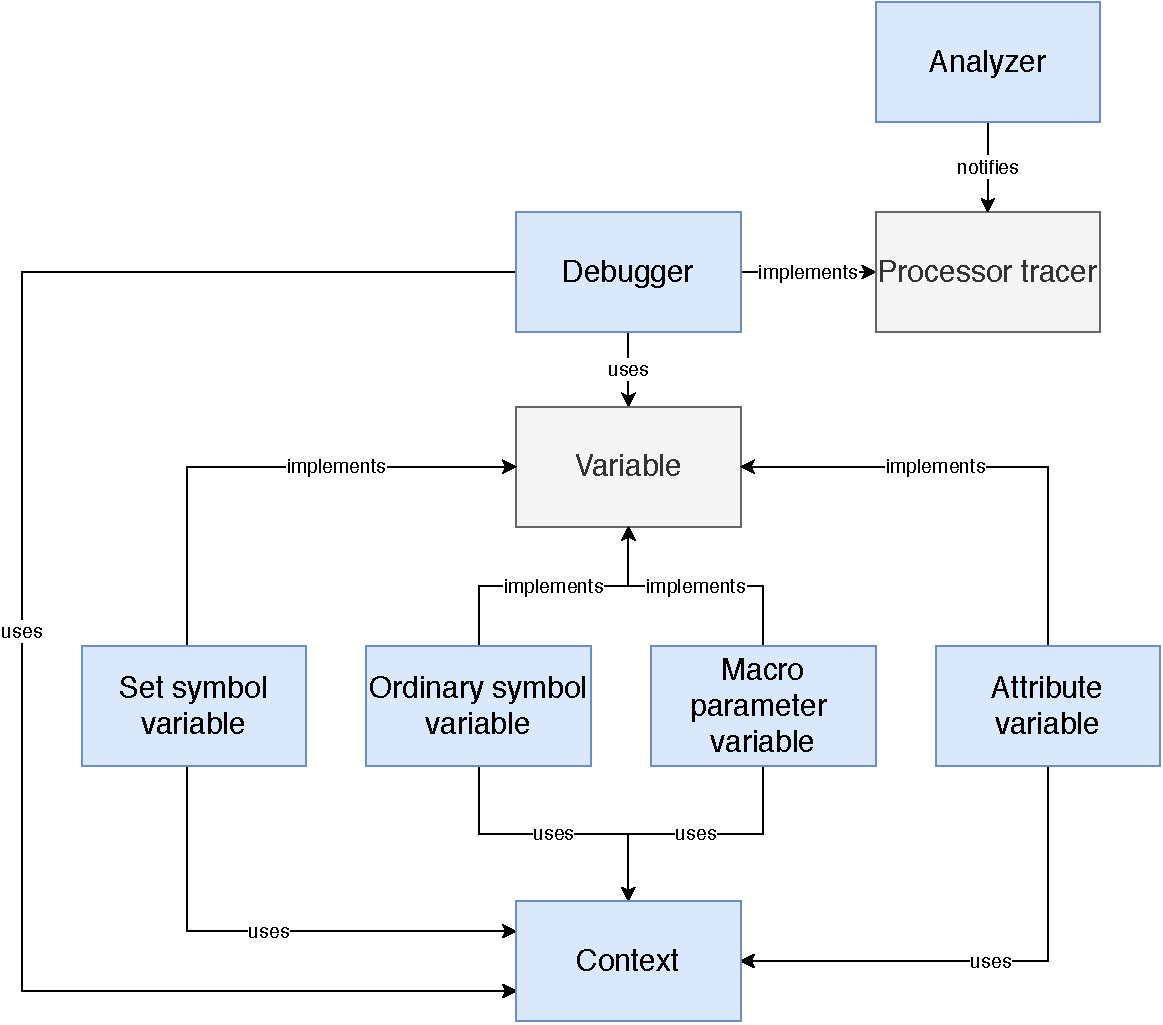
\includegraphics[width=\textwidth]{img/macro_tracer_arch}
	\caption{Architecture of macro tracer.}
	\label{macro_tracer_arch}
\end{figure}

Macro tracer architecture is shown in \cref{macro_tracer_arch}.

Debugger is a class that encapsulates all macro tracer functionality. It starts standard analysis that is provided by the analyzer component in a special thread. The debugger implements processor tracer interface which allows it to receive a notification every time when a statement is about to be processed.

It is also debugger responsibility to extract data from the context used by the analyzer and transform them to a form compatible with DAP.

Debugger uses interface variable which represents a variable as it is shown to the user --- most importantly it is a name-value pair. The variable interface has four implementations:
\begin{itemize}
	\item Set symbol variable
	\item Ordinary symbol variable
	\item Macro parameter variable
	\item Attribute variable
\end{itemize}
Each of the first three represent a HLASM symbol of certain type. They adapt the context representation of the symbols to DAP variables.

Attribute variable represents attributes of all types of symbols. It does not access context, it is only used by the rest of variables to show their attributes.

\section{Debugger}


The debugger component is the core of macro tracer implementation. When the user starts debugging, method \TT{launch} is called from the language server component. The debugger creates analyzer and starts analysis in a separate thread. The debugger implements processor tracer interface which only has one method \TT{statement}. The analyzer calls the \TT{statement} method every time when next statement is about to be processed.

This implementation makes it possible for debugger to stop the analysis using conditional variable. When it sees fit (e.g. when a breakpoint was hit), the debugger can put the thread to sleep and wait for further user interaction. At the same time, it notifies the language server through debug event consumer interface that the analyzer has stopped.

There are three important structures in DAP.
\begin{itemize}
	\item \textbf{Stack frame} Stack frame is one item in call stack. Each frame has name that is shown to the user and points to a line in source code. In macro tracer, each frame points either to the next instruction, to macro call or a COPY instruction.
	\item \textbf{Scope} Each stack frame may have scopes. A scope is simply a group of variables used to make them organized for the user. Macro tracer uses three scopes: Local variables, global variables and ordinary symbols.
	\item \textbf{Variable} Each scope has any number of variables. Each variable has a name and value. They may be further structured and have additional child variables. So DAP can be used to present arbitrary tree of variables to the user. \Cref{dap_nested_variables} shows an example regarding nested macro parameters.

\end{itemize}

\begin{listing}
	
	\begin{verbatim}
	MAC (foo,((bar,ex),am),ple,(lorem,ipsum))
	
	1: foo
	2: ((bar,ex),am)
	1: (bar,ex)
	1: bar
	2: ex
	2: am
	3: ple
	4: (lorem,ipsum)
	1: lorem
	2: ipsum
	
	\end{verbatim}
	\caption{An example how macro tracer leverages DAP nested variables. First line shows a macro call with a parameter. HLASM treats such parameters as nested arrays. Second part shows how such parameter is shown in VS Code using nested variables}
	\label{dap_nested_variables}
\end{listing}

While the thread is stopped, the editor sends requests to display informations about current context. It is the debugger responsibility to extract list of stack frames from the context, return list of scopes for each stack frame and list of variables for each scope. It does not have to deal with complexity of different types of set symbols and macro parameters, that is done by implementations of the variable interface.



\section{External Macro Libraries and COPY Members}
\label{sec:configuration}

The HLASM Language Support extension looks for locally stored members when a macro or COPY instruction is evaluated. The paths of these members are specified in two configuration files in the \TT{.hlasmplugin} folder of the currently open workspace:
\begin{itemize}
	\item  \TT{proc\_grps.json} defines \textbf{processor groups} by assigning a group name to a list of directories. Hence, the group name serves as a unique identifier of a HLASM library set defined by a list of directories.
	
	
	\item  \TT{pgm\_conf.json} provides a mapping between \textbf{programs} (open-code files) and processor groups. It specifies which list of directories is used with which source file. If a relative source file path is specified, it is relative to the current workspace.
\end{itemize}

Therefore, to use a predefined set of macro and copy members, do the following steps: 
\begin{enumerate}
	\item Enumerate the library directories in \TT{proc\_grps.json} and name them with an identifier; thus, create a new processor group.
	\item Use the identifier of the new processor group with the name of your source code file in \TT{pgm\_conf.json} to assign the library members to the program.
\end{enumerate}

The structure of the configuration is based on CA Endevor® SCM.


\begin{listing}
	\begin{verbatim}
{
  "pgroups": [
    {
      "name":"GROUP1",
      "libs": [
        "ASMMAC/",
        "C:/SYS.ASMMAC"
      ]
    },
    {
      "name":"GROUP2",
      "libs": [
        "G2MAC/",
        "C:/SYS.ASMMAC"
      ]
    }
  ]
}
	\end{verbatim}
	\caption{This example defines two processor groups, GROUP1 and GROUP2, and a list of directories to search for macros and COPY files.}
	\label{lst:ex1}
\end{listing}

\begin{listing}
	\begin{verbatim}
{
  "pgms": [
    {
      "program": "source",
      "pgroup": "GROUP1"
    },
    {
      "program": "asm_prg",
      "pgroup": "GROUP2"
    },
  ]
}
	\end{verbatim}
	\caption{Example \TT{proc\_grps.json} specifies that GROUP1 is used when working with \TT{source\_code.hlasm} and GROUP2 is used when working with \TT{second\_file.hlasm}}
	\label{lst:grps}
\end{listing}

An example configuration can be seen in \cref{lst:ex1} and \cref{lst:grps}. It describes two processor groups \TT{GROUP1}, \TT{GROUP2} and their respective mappings to programs \TT{source} and \TT{asm\_prg}. If you have the two configuration files configured as above and invoke the MAC1 macro from \TT{source}, the folder \TT{ASMMAC/} in the current workspace is searched for a file named exactly MAC1. If that file is not found, the folder \TT{C:/SYS.ASMMAC} is searched. If that search is unsuccessful too, an error displays that the macro does not exist.

Note that the macro \TT{MAC1} is searched in directories in order as they are listed in the configuration. 

To add a possibility to specify a custom extension for HLASM files in the workspace, {pgm\_conf.json} has an optional field \TT{alwaysRecognize}. It takes an array of wildcards and provides the following functionality:
\begin{itemize}
	\item All files matching these wildcards will always be recognized as HLASM files. Hence, the HLASM plugin will be automatically activated on all the matched files.
	\item If an extension wildcard is defined, all macro and copy files with such extension may be used in the source code. For example, with the extension wildcard \TT{*.hlasm}, a user may add macro MAC to his source code even if it is in a file called \TT{Mac.hlasm}.
\end{itemize}

\Cref{lst:alw} demonstrates the mentioned functionality. With this configuration file, processor group \TT{GROUP1} will be assigned to \TT{source} and \TT{source.hlasm} file as well. Also, macro and copy files in the \TT{lib} directory can be referenced and correctly recognized in the program without the \TT{.asm} extension.


\begin{listing}
	\begin{verbatim}
{
  "pgms": [
  {
    "program": "source",
    "pgroup": "GROUP1"
  }
  ],
   "alwaysRecognize" : ["*.hlasm", "libs/*.asm"]
}
	\end{verbatim}
	\caption{In this example, GROUP1 is used for all open code programs.}
	\label{lst:alw}
\end{listing}

Lastly, the program field in \TT{pgm\_conf.json} supports wildcards as well (see \cref{lst:wild}). This provides simplified use for users that share one processor group among all their programs.

\begin{listing}
	\begin{verbatim}
{
  "pgms": [
  {
    "program": "*",
    "pgroup": "GROUP1"  
  }
  ]
}
	\end{verbatim}
	\caption{In this example, GROUP1 is used for all open code programs.}
	\label{lst:wild}
\end{listing}



\end{document}
